\documentclass{article}
\usepackage[utf8]{inputenc}
\usepackage{amsmath}
\usepackage{graphicx}
\usepackage{subcaption}
\captionsetup{compatibility=false}
\usepackage[section]{placeins}
\usepackage{float}
\title{Assignment 3}
\author{Prashant Lawhatre (17510056)}
\date{20 September 2018}

\begin{document}

\maketitle

\section{Dilation}
    \subsection{ Set Difference}
    Let A=\{1 2 3 4 5 6\} and B=\{4 5 6 7 8 9\} $\implies$ C=A-B=[1 2 3]\\
    Let A=\{1 2 3 4 5 6\} and B=\{10\} $\implies$ C=A-B=[1 2 3 4 5 6]\\
    Let A=\{1 \} and B=\{4 5 6 7 8 9\} $\implies$ C=A-B=[1]\\
    \subsection{ Set complement}
    Let U=\{1 2 3 4 5 6\} and A=\{4 5 6 \} $\implies$ C=$A^c$=[1 2 3]\\
    Let U=\{\}(When U is not specified) and A=\{1 2 3\} $\implies$ C=$A^c$=[NaN] (Universal set not properly defined)\\
    Let U=\{4 5 6\} and B=\{4 5 6\} $\implies$ C=$A^c$=[ ] (null set)\\
    \subsection{Set reflection}
    Let A=\{1 2 3 4 5 6\} $\implies$ C=$\hat{A}$=[6 5 4 3 2 1]\\
    Let A=\{4 5 6\} $\implies$ C=$\hat{A}$=[6 5 4 ]\\
    Let A=\{1 2 3\} $\implies$ C=$\hat{A}$=[3 2 1]\\
    \subsection{Set A subset of Set B}
    Let A=\{1 2 3\} and B=\{1 2 3 4 5 6\} $\implies$ C=A $\subset$ B=1 (boolean logic)\\
    Let A=\{1 2 3 4 5 6\} and B=\{10\} $\implies$ C=A $\subset$ B=0 (boolean logic)\\
    Let A=\{1 \} and B=\{4 5 6 7 8 9\} $\implies$ C=A $\subset$ B=0 (boolean logic)\\
    \subsection{Set A intersection Set B}
    Let A=\{1 2 3 4 5 6\} and B=\{4 5 6 7 8 9\} $\implies$ C=A $\cap$ B=[4 5 6]\\
    Let A=\{1 2 3\} and B=\{8 9 0\} $\implies$ C=A $\cap$ B=[ ] (null set)\\
    Let A=\{1 \} and B=\{1 4 5 6 7 8 9\} $\implies$ C=A $\cap$ B=[1 ]\\
    \subsection{ Set A union Set B}
    Let A=\{1 2 3\} and B=\{4 5 6\} $\implies$ C=A $\cup$ B=[1 2 3 4 5 6]\\
    Let A=\{1 2 3\} and B=\{8 9 0\} $\implies$ C=A $\cup$ B=[1 2 3 8 9 0]\\
    Let A=\{1 \} and B=\{4 5 6 7 8 9\} $\implies$ C=A $\cup$ B=[1 4 5 6 7 8 9]\\
    \subsection{Set translation}
    Let \[
    A=
    \begin{bmatrix} 
    1 & 2 \\
    3 & 4 \\
    5 & 6
    \end{bmatrix}
    \]
     and \[h=\begin{bmatrix} 1 & 1
     \end{bmatrix}
     \]
     $\implies$ 
     C=$A_h$=\[
     \begin{bmatrix}
     2 & 3\\
     4 & 5\\
     6 & 7
     \end{bmatrix}
     \]
     \subsection{Dilation definition1}
     Problem solved in the class\\
     Let \[
    A=
    \begin{bmatrix} 
    1 & 1
    \end{bmatrix}
    \]
     and \[B=\begin{bmatrix} 0 & -1\\
     0 & 2
     \end{bmatrix}
     \]
     $\implies$ C=A $\oplus$ B=
     \[
     \begin{bmatrix}
     1 & 0\\
     1 & 3
     \end{bmatrix}
     \]
     \subsection{Dilation definition2}
     Let \[
    A=
    \begin{bmatrix} 
    1 & 1
    \end{bmatrix}
    \]
     and \[B=\begin{bmatrix} 0 & -1\\
     0 & 2
     \end{bmatrix}
     \]
     $\implies$ C=A $\oplus$ B=
     \[
     \begin{bmatrix}
     1 & 0\\
     1 & 3
     \end{bmatrix}
     \]
     \subsection{Dilation definition3}
     Let \[
    A=
    \begin{bmatrix} 
    1 & 1
    \end{bmatrix}
    \]
     and \[B=\begin{bmatrix} 0 & -1\\
     0 & 2
     \end{bmatrix}
     \]
     $\implies$ C=A $\oplus$ B=
     \[
     \begin{bmatrix}
     1 & 0\\
     1 & 3
     \end{bmatrix}
     \]
     \newline
     REMARK: Dilation calculated using all the three formulas is same.
\section{Image Halftoning}
Let \[
    \alpha=
    \begin{bmatrix} 
    \alpha1 &
    \alpha2 &
    \alpha3 &
    \alpha4 &
    \alpha5 &
    \alpha6 &
    \end{bmatrix}
    \]
    \\
    and\\
%%%%%%%%%%%%%%%%%%%
\begin{figure}[h!]
  \centering
  \begin{subfigure}[b]{0.4\linewidth}
    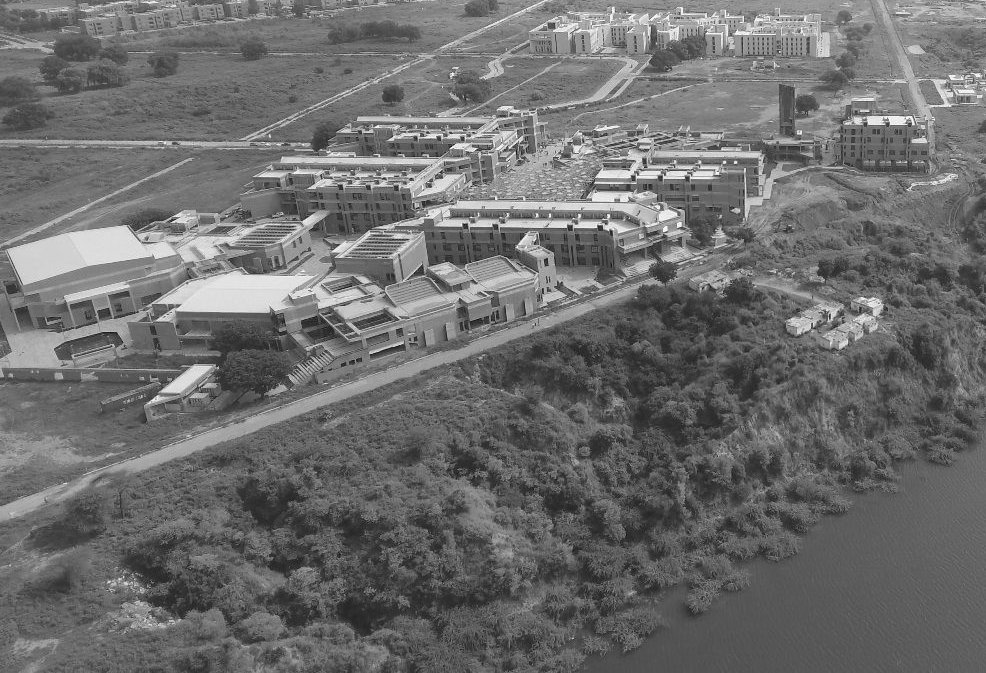
\includegraphics[width=\linewidth]{campus.png}
     \caption{campus}
  \end{subfigure}
  \begin{subfigure}[b]{0.4\linewidth}
    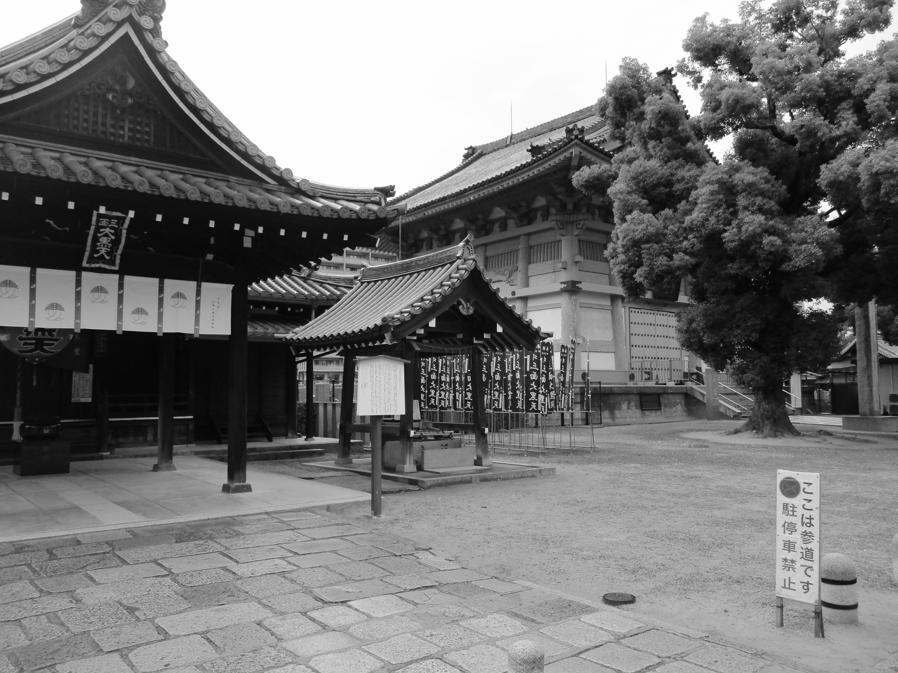
\includegraphics[width=\linewidth]{1_user.jpg}
     \caption{1{\_}user}
  \end{subfigure}
  \begin{subfigure}[b]{0.4\linewidth}
    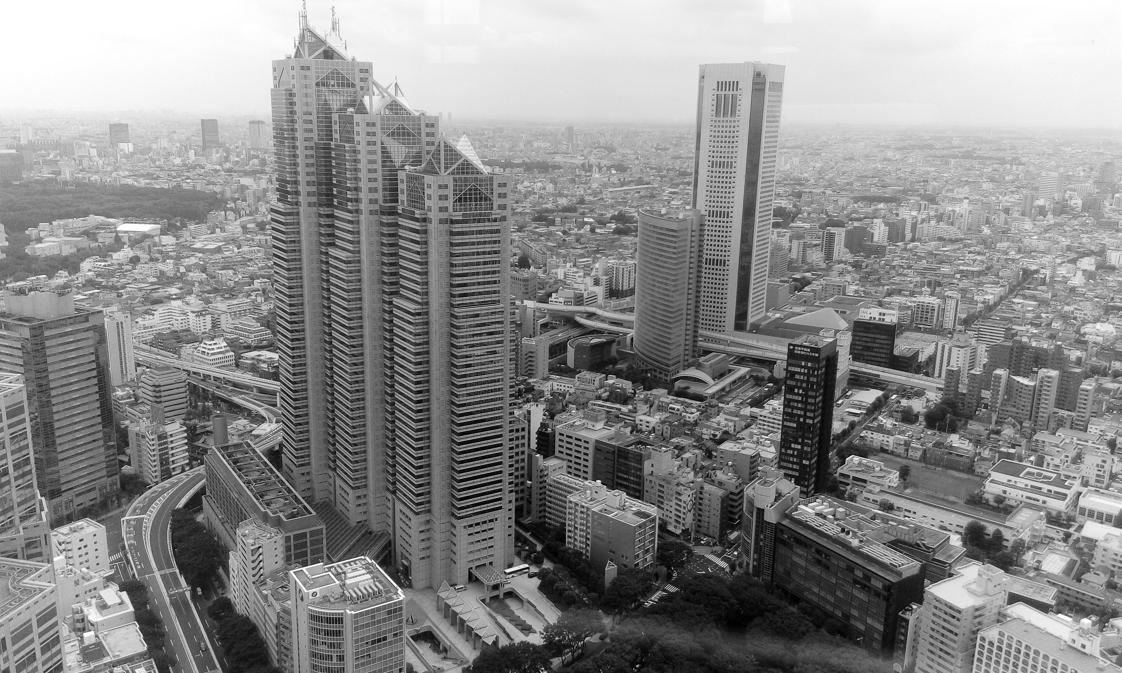
\includegraphics[width=\linewidth]{2_user.jpg}
     \caption{2{\_}user}
  \end{subfigure}
  \begin{subfigure}[b]{0.4\linewidth}
    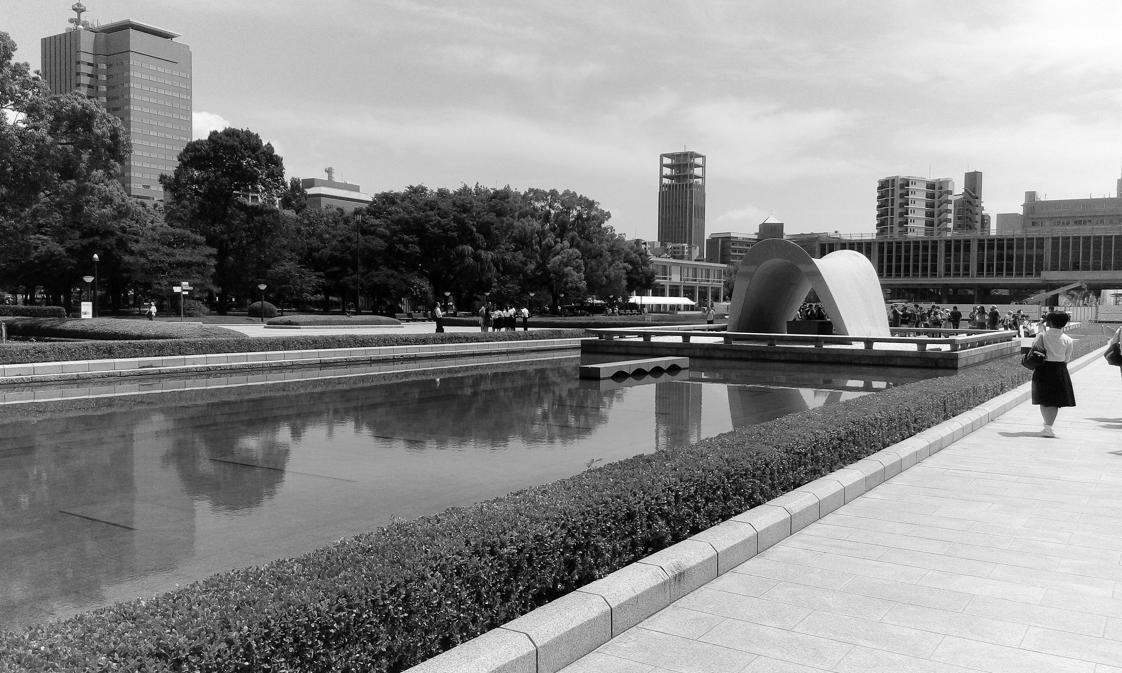
\includegraphics[width=\linewidth]{3_user.jpg}
     \caption{3{\_}user}
  \end{subfigure}
  \caption{Input Images to the code}
\end{figure}
%%%%%%%%%%%%%%%%%%%
\subsection{Thresholding}
\begin{enumerate}
    \item Input Image $\longrightarrow$ campus
    \begin{figure}[H]
        \centering
        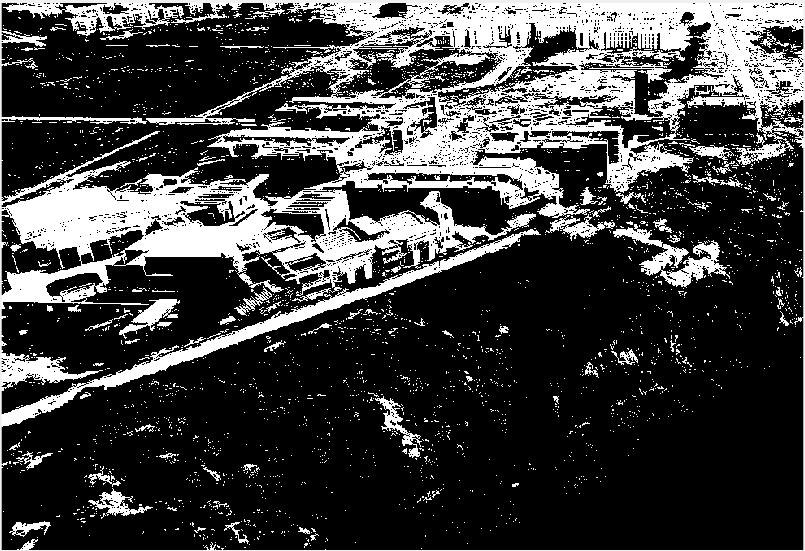
\includegraphics[width=0.75\linewidth]{1.png}
        \caption{Image after thresholding}
        \label{fig:Image after thresholding}
    \end{figure}
    \[
    \alpha=
    \begin{bmatrix} 
     62.3617 &
     62.9058 &
     62.7899 &
     68.3735 &
     0.3529 &
     0.00010357 &
    \end{bmatrix}
    \]
    \item Input Image $\longrightarrow$ 1{\_}user
    \begin{figure}[H]
        \centering
        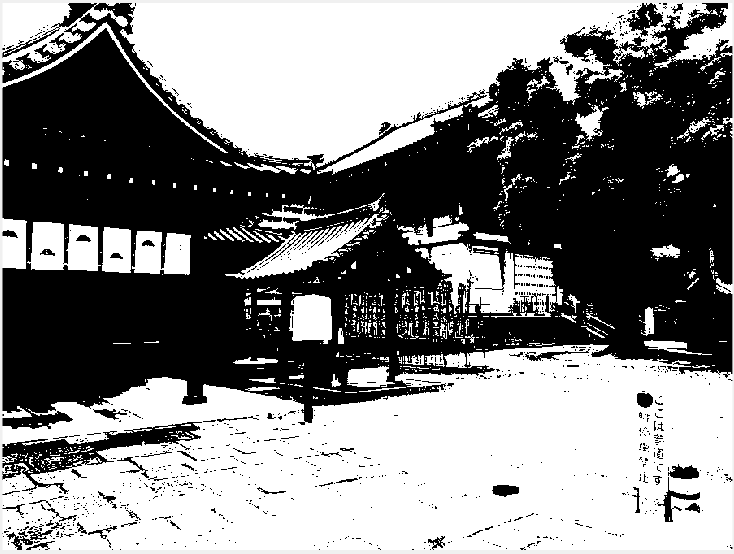
\includegraphics[width=0.75\linewidth]{2.png}
        \caption{Image after thresholding}
        \label{fig:Image after thresholding}
    \end{figure}
    \[
    \alpha=
    \begin{bmatrix} 
    -130.02183 &
    130.4281 &
    130.69 &
    126.3663 &
    -254.4314 &
    0.0006300905 &
    \end{bmatrix}
    \]
    \item Input Image $\longrightarrow$ 2{\_}user
    \begin{figure}[H]
        \centering
        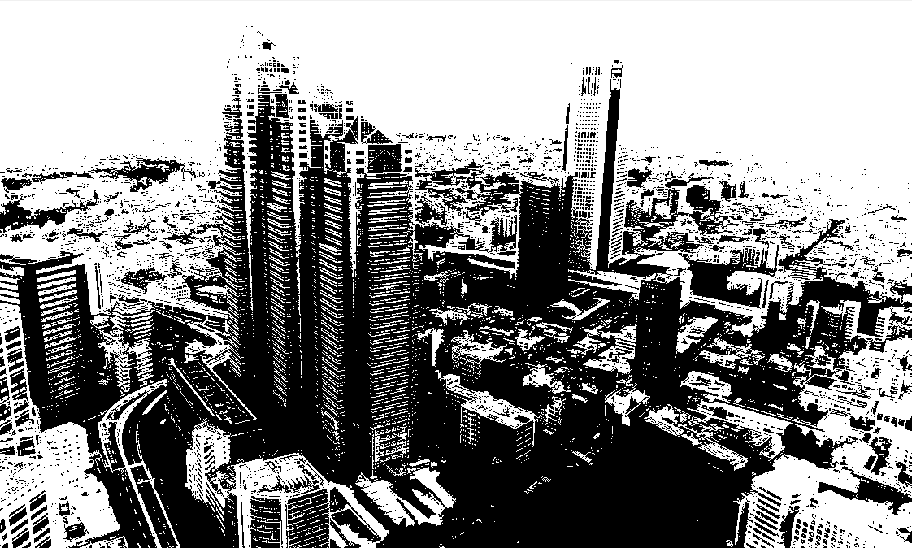
\includegraphics[width=0.75\linewidth]{3.png}
        \caption{Image after thresholding}
        \label{fig:Image after thresholding}
    \end{figure}
    \[
    \alpha=
    \begin{bmatrix} 
     -139.0461 &
     139.3274 &
     139.5907 &
     135.1631 &
     -254.2863 &
     0.0005157546 &
    \end{bmatrix}
    \]
    \item Input Image $\longrightarrow$ 3{\_}user
    \begin{figure}[H]
        \centering
        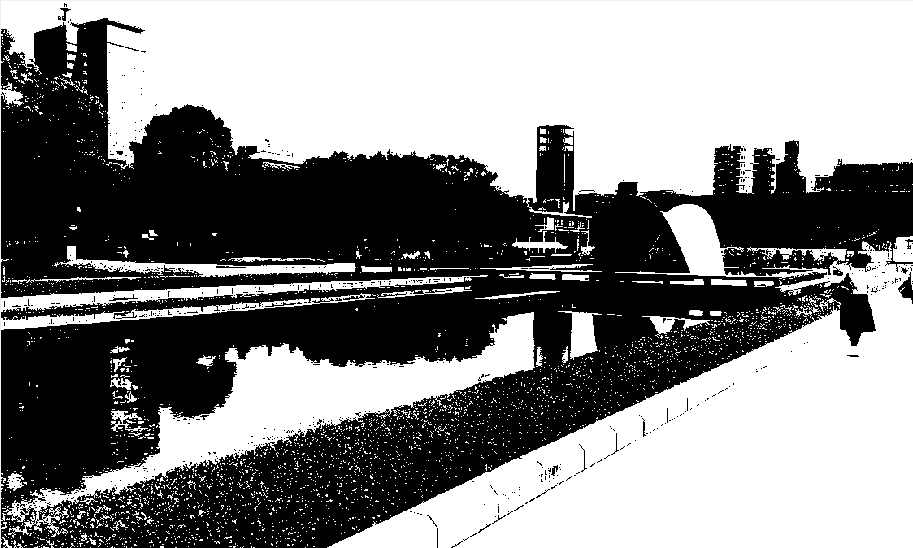
\includegraphics[width=0.75\linewidth]{4.png}
        \caption{Image after thresholding}
        \label{fig:Image after thresholding}
    \end{figure}
    \[
    \alpha=
    \begin{bmatrix} 
     -62.3617 &
     62.9058 &
     62.7899 &
     68.3735 &
     0.352941 &
     0.00010357 &
    \end{bmatrix}
    \]
    \end{enumerate}
    %%%%%%%%%%
    \subsection{Random noise Binarization}
    \begin{enumerate}
        \item Input Image $\longrightarrow$ campus
    \begin{figure}[H]
        \centering
        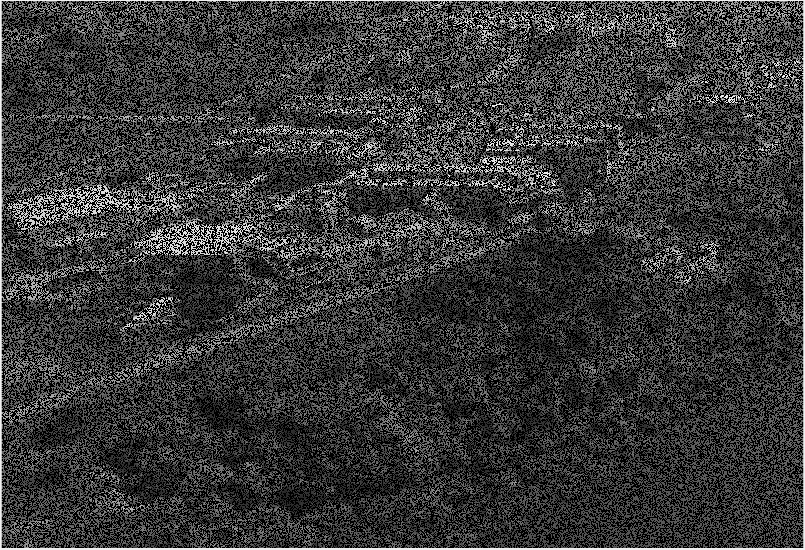
\includegraphics[width=0.75\linewidth]{5.png}
        \caption{Image after addition of random noise}
        \label{fig:Image after addition of random noise}
    \end{figure}
    \begin{figure}[H]
        \centering
        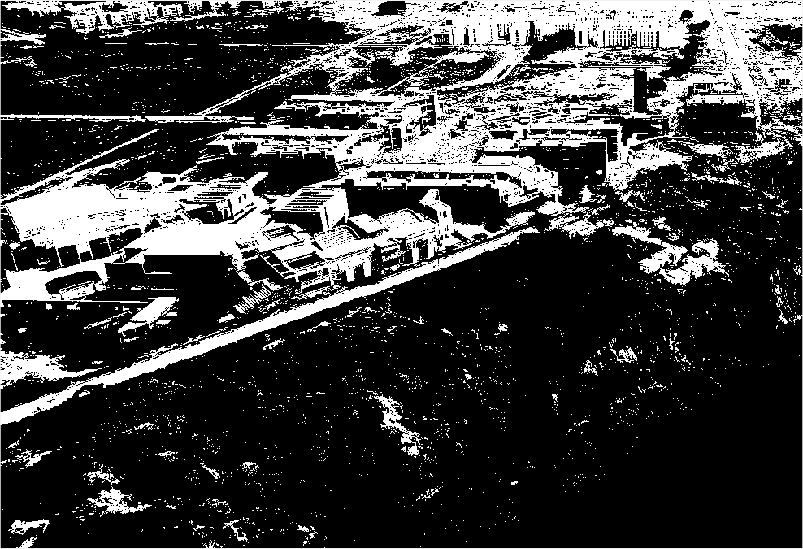
\includegraphics[width=0.75\linewidth]{6.png}
        \caption{Image after Binarization}
        \label{fig:Image after Binarization}
    \end{figure}
    \[
    \alpha=
    \begin{bmatrix} 
     -62.3617 &
     62.9058 &
     62.7899 &
     68.3735 &
     0.352941 &
     0.00010357 &
    \end{bmatrix}
    \]
    %
    \\
    \item Input Image $\longrightarrow$ 1{\_}user
    \begin{figure}[H]
        \centering
        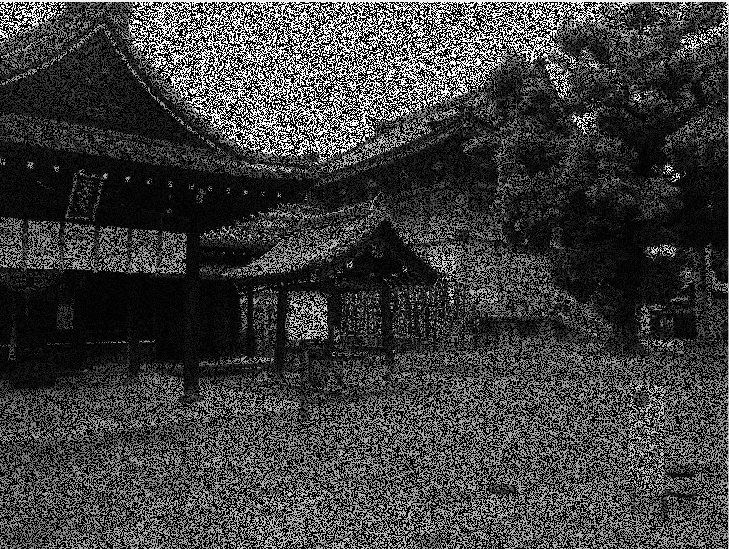
\includegraphics[width=0.75\linewidth]{7.png}
        \caption{Image after addition of random noise}
        \label{fig:Image after addition of random noise}
    \end{figure}
    \begin{figure}[H]
        \centering
        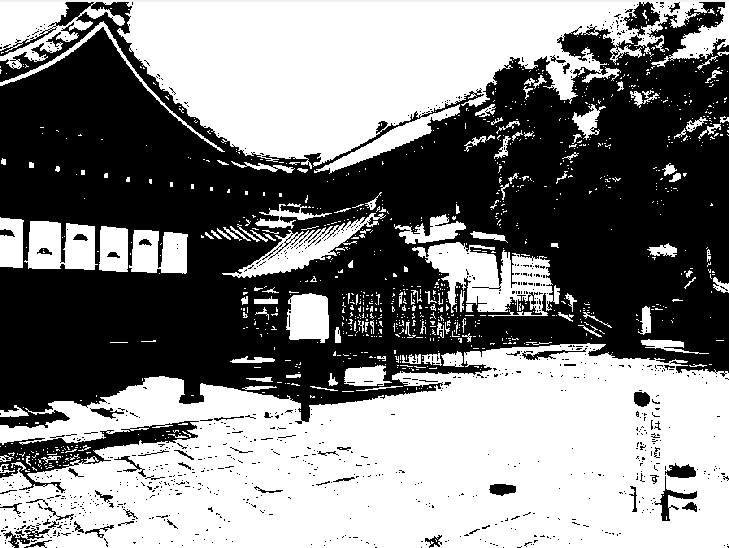
\includegraphics[width=0.75\linewidth]{8.png}
        \caption{Image after Binarization}
        \label{fig:Image after Binarization}
    \end{figure}
    \[
    \alpha=
    \begin{bmatrix} 
     -130.02183 &
     130.4281 &
     130.69 &
     126.3663 &
     -254.4314 &
     0.000063000905 &
    \end{bmatrix}
    \]
    \\
    \item Input Image $\longrightarrow$ 2{\_}user
    \begin{figure}[H]
        \centering
        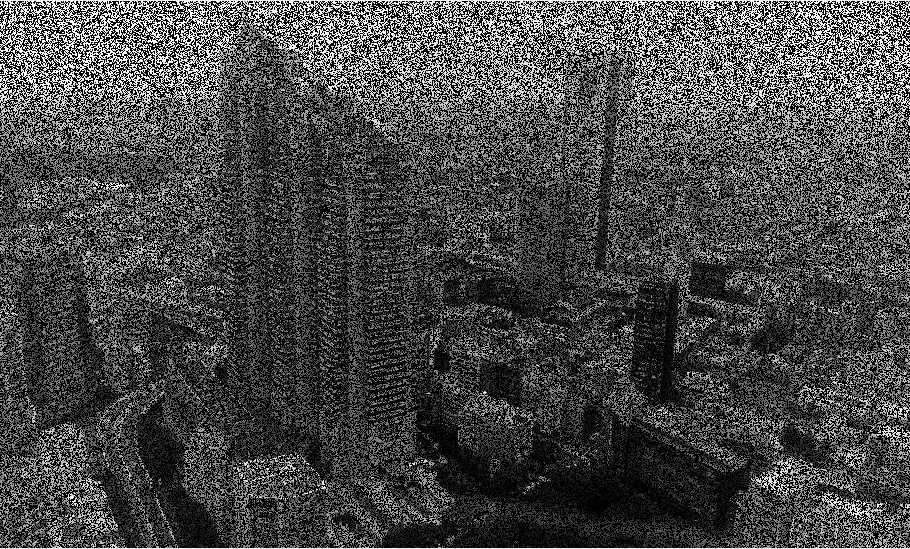
\includegraphics[width=0.75\linewidth]{9.png}
        \caption{Image after addition of random noise}
        \label{fig:Image after addition of random noise}
    \end{figure}
    \begin{figure}[H]
        \centering
        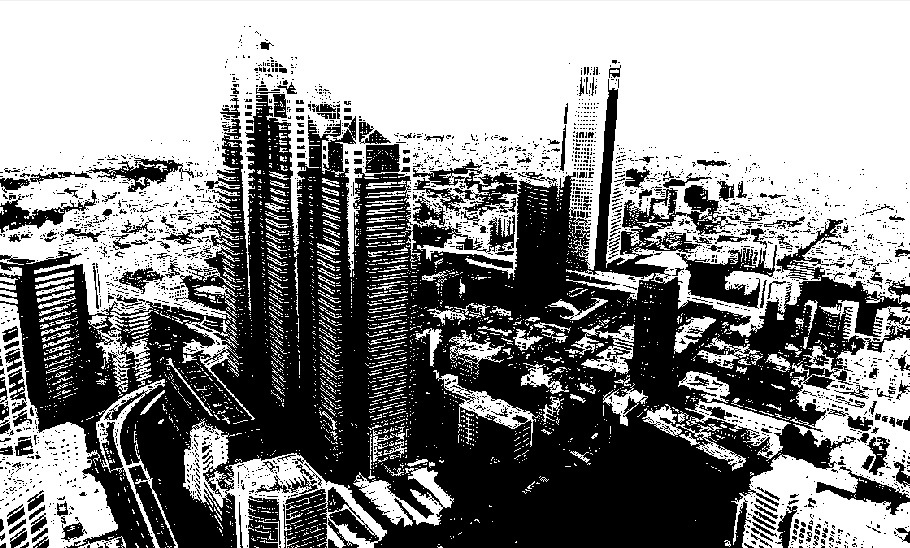
\includegraphics[width=0.75\linewidth]{10.png}
        \caption{Image after Binarization}
        \label{fig:Image after Binarization}
    \end{figure}
    \[
    \alpha=
    \begin{bmatrix} 
     -139.0461 &
     139.3274 &
     139.5907 &
     135.1631 &
     -254.2863 &
     0.0005157546 &
    \end{bmatrix}
    \]
    %
    \newpage
    \item Input Image $\longrightarrow$ campus
    \begin{figure}[H]
        \centering
        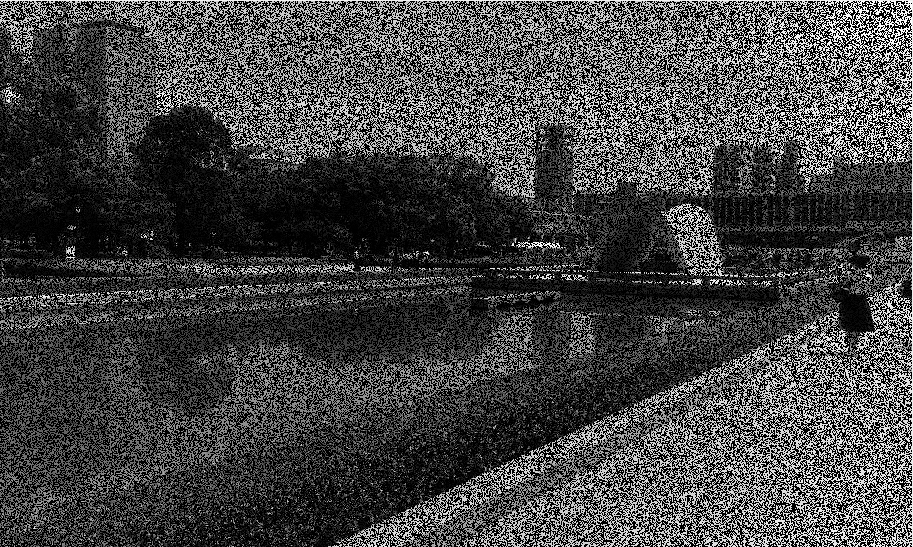
\includegraphics[width=0.75\linewidth]{11.png}
        \caption{Image after addition of random noise}
        \label{fig:Image after addition of random noise}
    \end{figure}
    \begin{figure}[H]
        \centering
        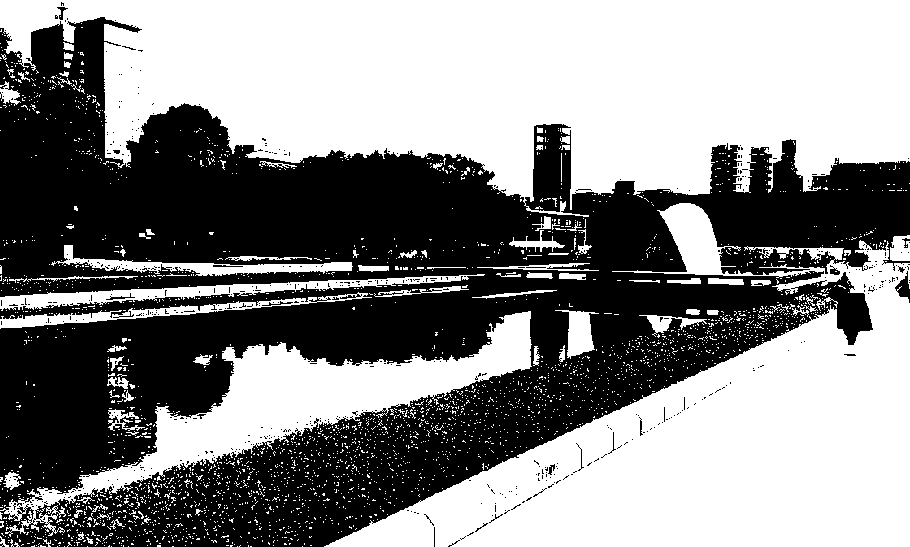
\includegraphics[width=0.75\linewidth]{12.png}
        \caption{Image after Binarization}
        \label{fig:Image after Binarization}
    \end{figure}
    \[
    \alpha=
    \begin{bmatrix} 
     -135.296 &
     135.5374 &
     135.8314 &
     131.0317 &
     -254.0863 &
     0.0005100184 &
    \end{bmatrix}
    \]
    \end{enumerate}
    \subsection{Ordered Dithering}
    For all the images processed, following where the index and threshold matrices. 
    Index Matrices
    \[
    i2=
    \begin{bmatrix} 
     1	& 2 \\
3	& 0 
    \end{bmatrix}
    \]
     \[
    i4=
    \begin{bmatrix} 
     5	& 9	& 6	& 10 \\
13	& 1	& 14 &	2 \\
7	& 11	& 4	& 8 \\
15	& 3	& 12	& 0 \\
    \end{bmatrix}
    \]
     \[
    i8=
    \begin{bmatrix} 
     21	& 37	& 25	& 41	& 22	& 38	& 26	& 42 \\
53	& 5	& 57	& 9	& 54	& 6	& 58 &	10 \\
29	& 45	& 17	& 33	& 30	& 46	& 18	& 34\\
61	& 13	& 49	& 1	& 62	& 14	& 50	& 2 \\
23	& 39	& 27	& 43	& 20	& 36	& 24	& 40\\
55	& 7	& 59	& 11	& 52	& 4	& 56	& 8 \\
31	& 47	& 19	& 35	& 28	& 44	& 16	& 32 \\
63	& 15	& 51	& 3	& 60	& 12	& 48	& 0 \\
    \end{bmatrix}
    \] 
    Threshold Matrices
    \[
    t2=
    \begin{bmatrix} 
    95.625 &	159.375 \\
223.125	& 31.875 
    \end{bmatrix}
    \]
    \[
    t4=
    \begin{bmatrix} 
    87.65625 &	151.40625 & 103.59375 & 167.34375 \\
215.15625 &	23.90625 &	231.09375 &	39.84375 \\
119.53125 &	183.28125 &	71.71875 &	135.46875 \\
247.03125 &	55.78125 &	199.21875 &	7.96875 \\
    \end{bmatrix}
    \]
    \[
    t8=
    \begin{bmatrix} 
    85.66 &	149.41 &	101.60 &	165.35 &	89.64 &	153.39 &	105.58 &	169.33 \\
213.16 &	21.91 &	229.10 &	37.85 &	217.14 &	25.89 &	233.08 &	41.83 \\
117.53 &	181.28 &	69.72 &	133.47 &	121.52 &	185.27 &	73.71 &	137.46 \\
245.03 &	53.78 &	197.22 &	5.97 &	249.02 &	57.77 &	201.21 &	9.96 \\
93.63 &	157.38 &	109.57 &	173.32 &	81.67 &	145.42 &	97.61 &	161.36 \\
221.13 &	29.88 &	237.07 &	45.82 &	209.17 &	17.92 &	225.11 &	33.86 \\
125.50 &	189.25 &	77.69 &	141.44 &	113.55 &	177.30 &	65.74 &	129.49 \\
253.00 &	61.75 &	205.19 &	13.94 &	241.05 &	49.80 &	193.24 &	1.99 \\
    \end{bmatrix}
    \]
    \begin{enumerate}
    \item Input Image $\longrightarrow$ campus
    \newline
    For t2 matrix
    \[
    \alpha=
    \begin{bmatrix} 
     0.0110 &	113.6441 &	104.9981 &	125.9509 &	90	& 0.0003
    \end{bmatrix}
    \]
    For t4 matrix
    \[
    \alpha=
    \begin{bmatrix} 
      -0.0446 &	113.7263 &	104.9625 &	126.0115 &	90 &	0.0003 
    \end{bmatrix}
    \]
    For t8 matrix
    \[
    \alpha=
    \begin{bmatrix} 
      -0.0711 &	113.7557 &	105.0047 &	126.0203 &	90 &	0.0003
    \end{bmatrix}
    \]
    \begin{figure}[H]
        \centering
        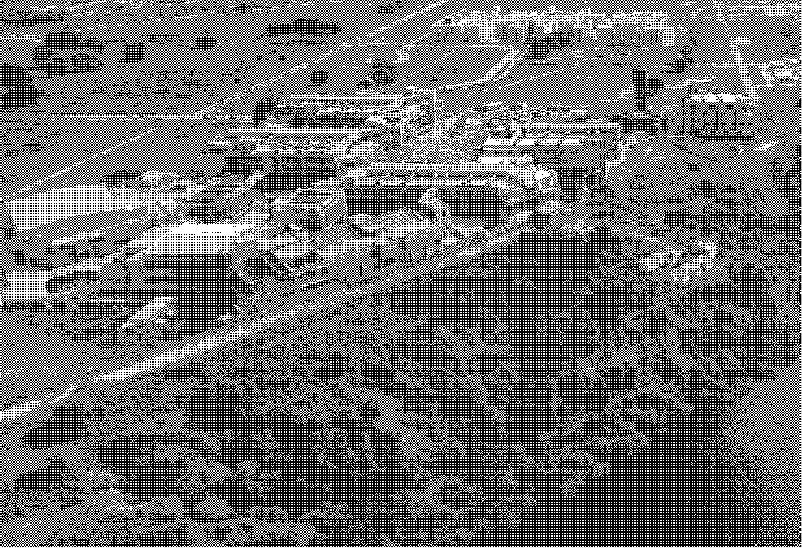
\includegraphics[width=0.75\linewidth]{311.png}
        \caption{Image after Dithering with t2 matrix}
        \label{fig:Image after Dithering with t2 matrix}
    \end{figure}
    \begin{figure}[H]
        \centering
        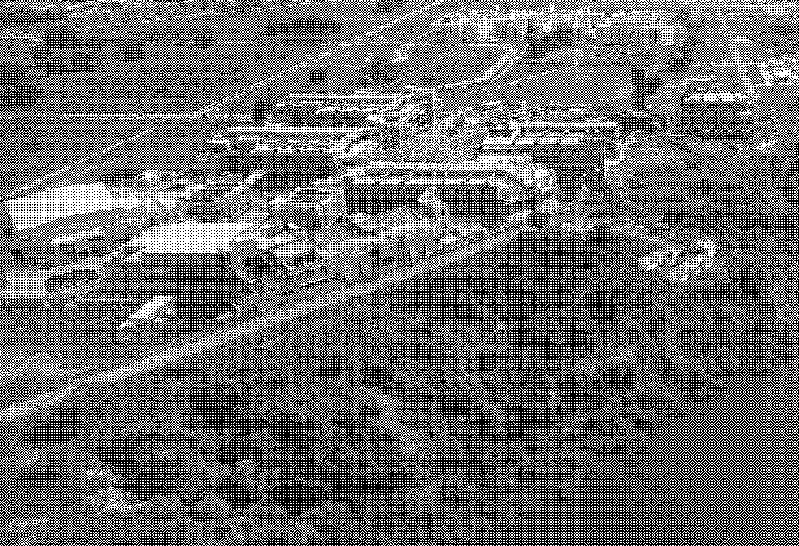
\includegraphics[width=0.75\linewidth]{312.png}
        \caption{Image after Dithering with t4 matrix}
        \label{fig:Image after Dithering with t2 matrix}
    \end{figure}
    \begin{figure}[H]
        \centering
        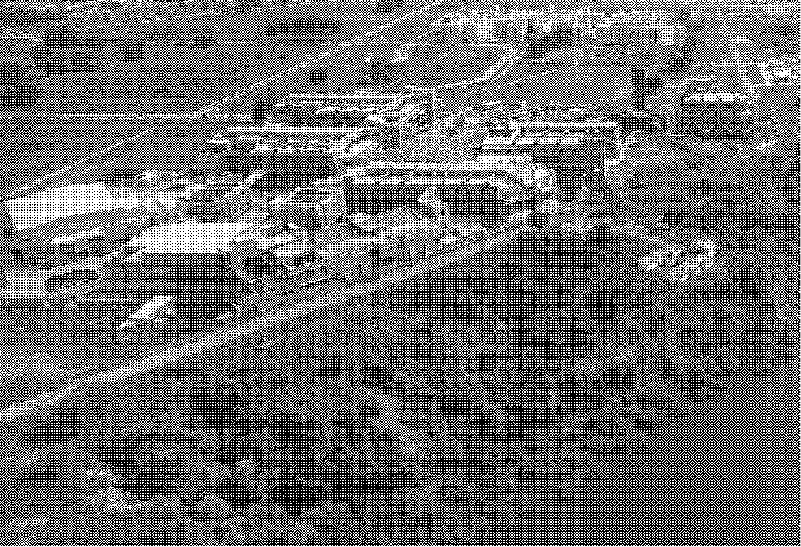
\includegraphics[width=0.75\linewidth]{313.png}
        \caption{Image after Dithering with t8 matrix}
        \label{fig:Image after Dithering with t8 matrix}
    \end{figure}
    \item Input Image $\longrightarrow$ 1{\_}user
        \newline
    For t2 matrix
    \[
    \alpha=
    \begin{bmatrix} 
    0.7954 &	80.1650 &	78.5373 &	93.7523 &	145 &	0.0003 
    \end{bmatrix}
    \]
    For t4 matrix
    \[
    \alpha=
    \begin{bmatrix} 
      -0.3396 &	82.3677 &	80.5479 &	95.3697 &	145 &	0.0003
    \end{bmatrix}
    \]
    For t8 matrix
    \[
    \alpha=
    \begin{bmatrix} 
      -0.1028 &	82.3852 &	80.5514 &	95.4292 &	145 &	0.0003
    \end{bmatrix}
    \]
    \begin{figure}[H]
        \centering
        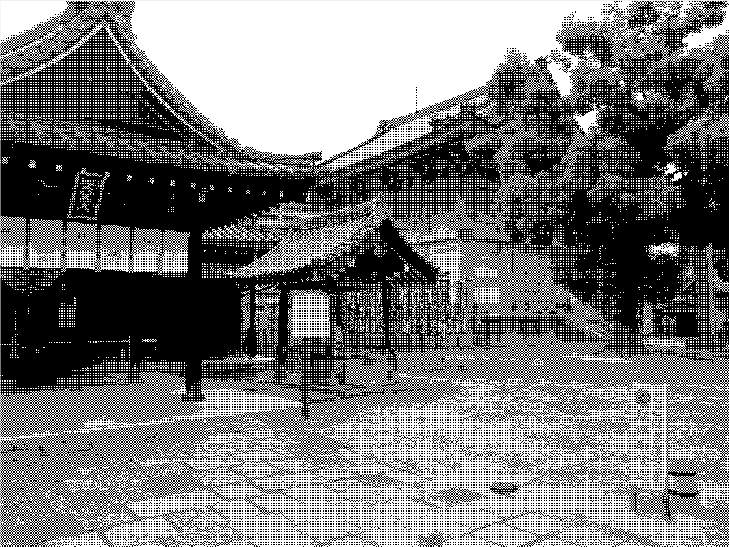
\includegraphics[width=0.75\linewidth]{321.png}
        \caption{Image after Dithering with t2 matrix}
        \label{fig:Image after Dithering with t2 matrix}
    \end{figure}
    \begin{figure}[H]
        \centering
        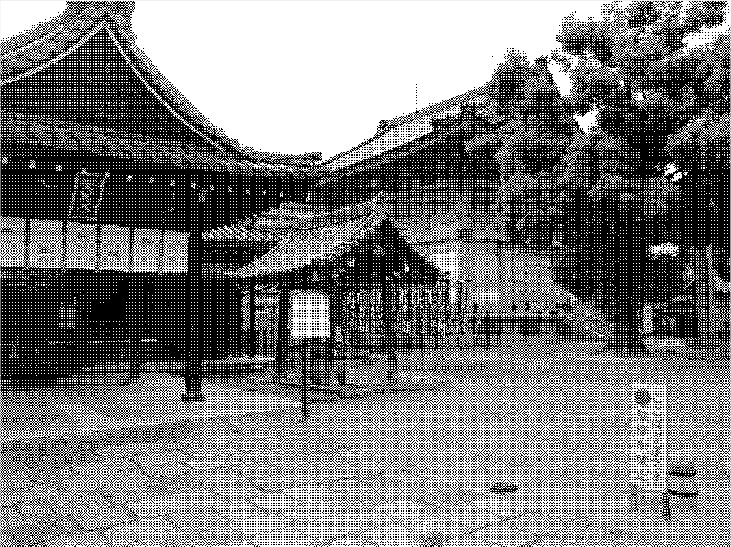
\includegraphics[width=0.75\linewidth]{322.png}
        \caption{Image after Dithering with t4 matrix}
        \label{fig:Image after Dithering with t2 matrix}
    \end{figure}
    \begin{figure}[H]
        \centering
        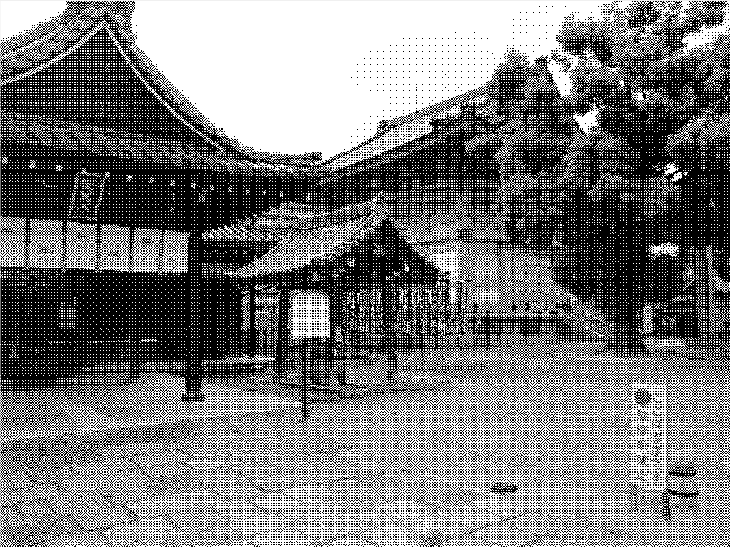
\includegraphics[width=0.75\linewidth]{323.png}
        \caption{Image after Dithering with t8 matrix}
        \label{fig:Image after Dithering with t8 matrix}
    \end{figure}
    \item Input Image $\longrightarrow$ 2{\_}user
       \newline
    For t2 matrix
    \[
    \alpha=
    \begin{bmatrix} 
     -2.3736 &	90.9633 &	92.9450 &	96.7172 &	182 &	0.0003 
    \end{bmatrix}
    \]
    For t4 matrix
    \[
    \alpha=
    \begin{bmatrix} 
      -0.0985 &	92.5632 &	93.8796 &	98.7433 &	182 &	0.0003 
    \end{bmatrix}
    \]
    For t8 matrix
    \[
    \alpha=
    \begin{bmatrix} 
      0.0114 &	92.6321 &	93.9389 &	98.8261 &	182 &	0.0003 
    \end{bmatrix}
    \]
    \begin{figure}[H]
        \centering
        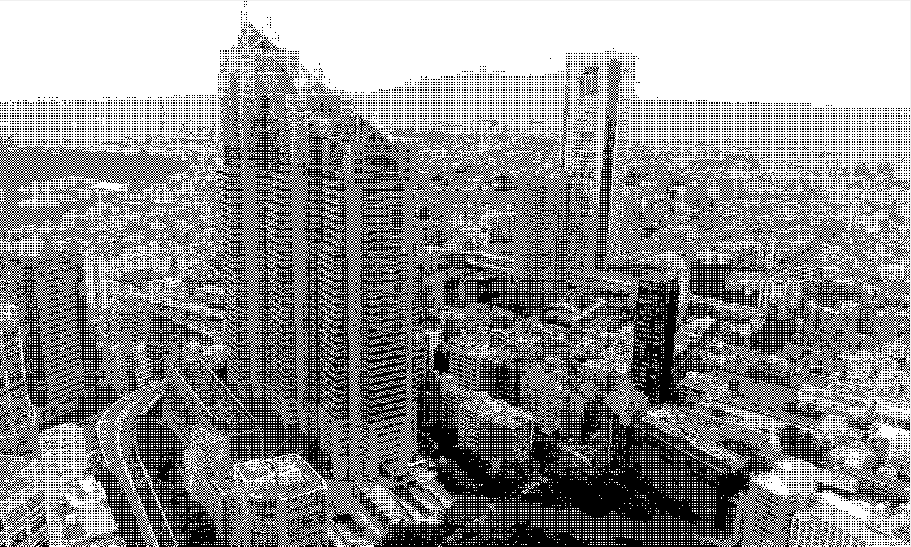
\includegraphics[width=0.75\linewidth]{331.png}
        \caption{Image after Dithering with t2 matrix}
        \label{fig:Image after Dithering with t2 matrix}
    \end{figure}
    \begin{figure}[H]
        \centering
        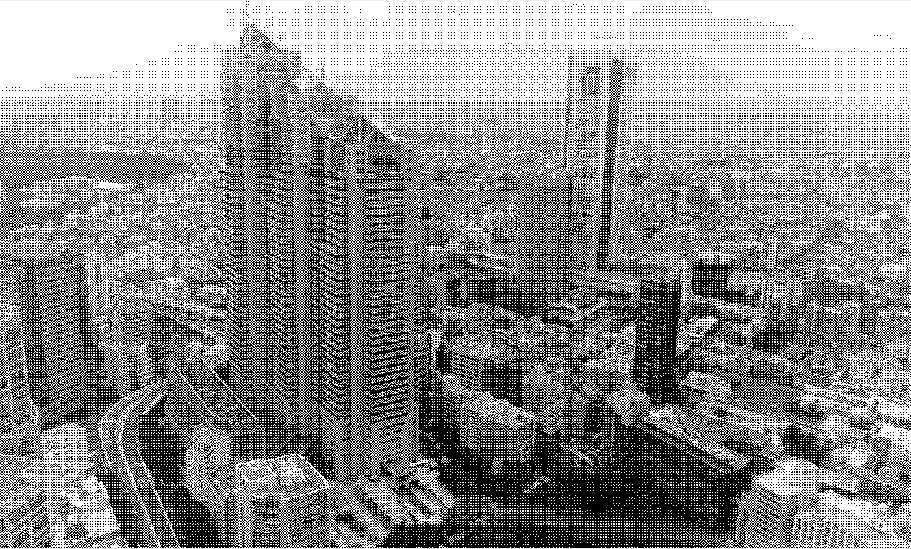
\includegraphics[width=0.75\linewidth]{332.png}
        \caption{Image after Dithering with t4 matrix}
        \label{fig:Image after Dithering with t2 matrix}
    \end{figure}
    \begin{figure}[H]
        \centering
        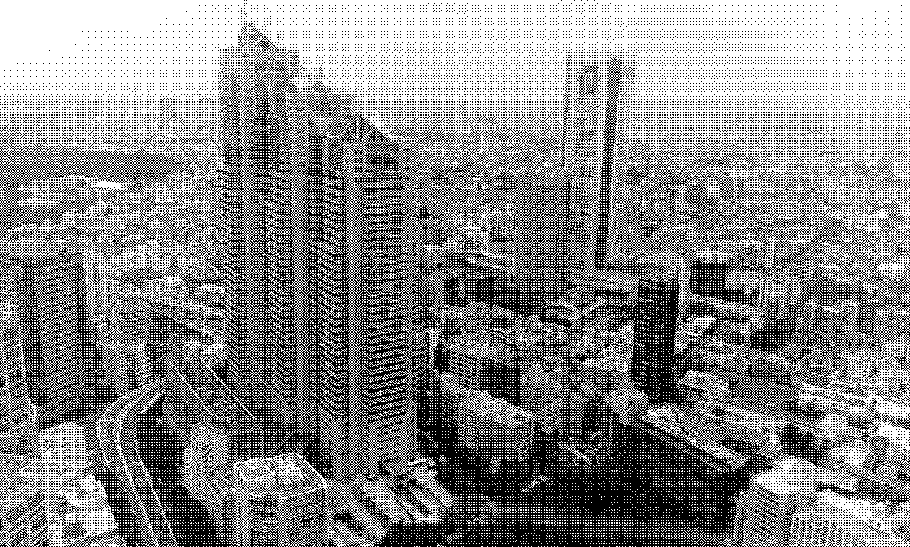
\includegraphics[width=0.75\linewidth]{333.png}
        \caption{Image after Dithering with t8 matrix}
        \label{fig:Image after Dithering with t8 matrix}
    \end{figure}
    \item Input Image $\longrightarrow$ 3{\_}user
        \newline
    For t2 matrix
    \[
    \alpha=
    \begin{bmatrix} 
     3.2266 &	84.8967 &	87.2740 &	93.4432 &	-22	0.0001
    \end{bmatrix}
    \]
    For t4 matrix
    \[
    \alpha=
    \begin{bmatrix} 
     0.1539 &	84.2340 &	87.7616 &	91.9374 &	-22	0.0001 
    \end{bmatrix}
    \]
    For t8 matrix
    \[
    \alpha=
    \begin{bmatrix} 
      0.1164 &	84.1998 &	87.7271 &	91.9079 &	-22 &	0.0001  
    \end{bmatrix}
    \]
    \begin{figure}[H]
        \centering
        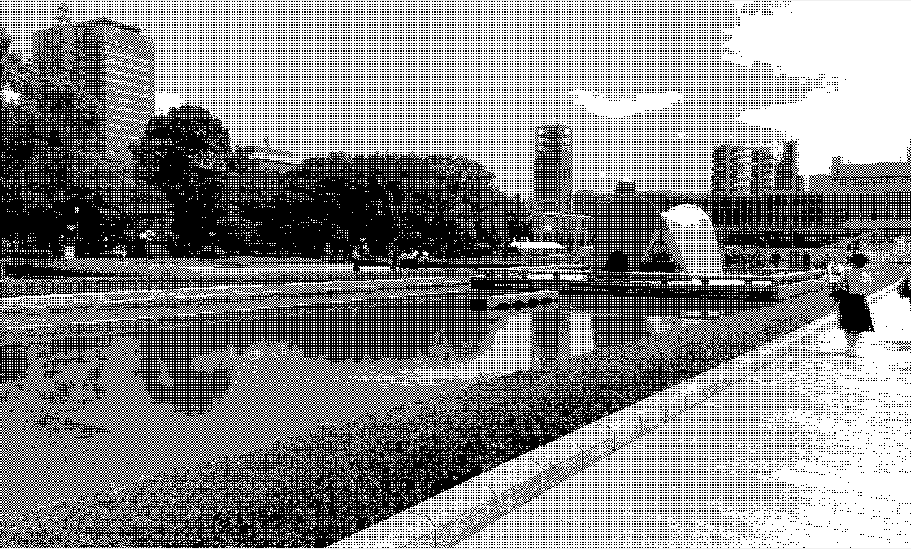
\includegraphics[width=0.75\linewidth]{341.png}
        \caption{Image after Dithering with t2 matrix}
        \label{fig:Image after Dithering with t2 matrix}
    \end{figure}
    \begin{figure}[H]
        \centering
        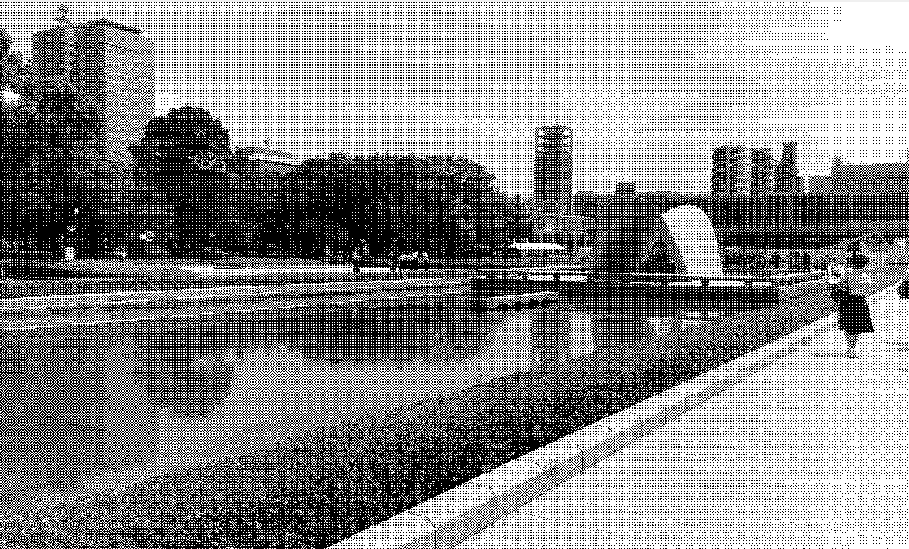
\includegraphics[width=0.75\linewidth]{342.png}
        \caption{Image after Dithering with t4 matrix}
        \label{fig:Image after Dithering with t2 matrix}
    \end{figure}
    \begin{figure}[H]
        \centering
        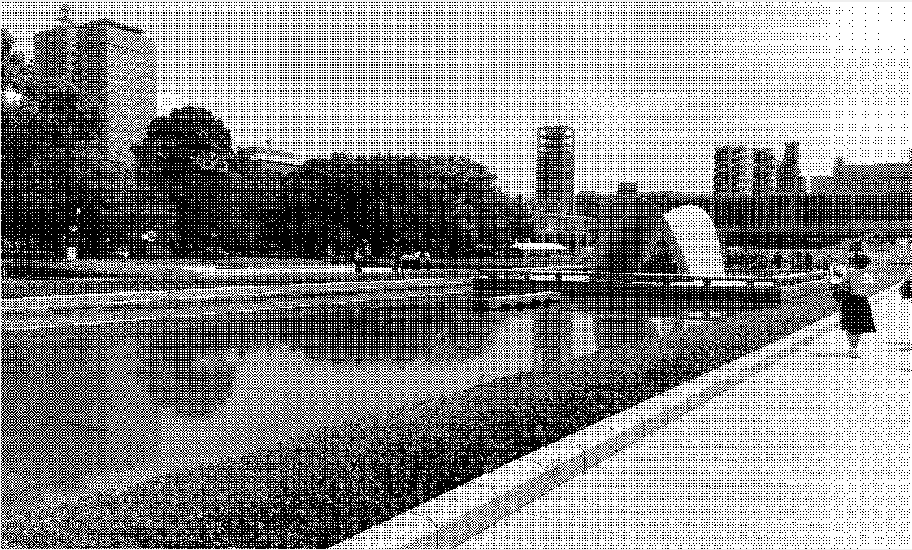
\includegraphics[width=0.75\linewidth]{343.png}
        \caption{Image after Dithering with t8 matrix}
        \label{fig:Image after Dithering with t8 matrix}
    \end{figure}
    \end{enumerate}
    \subsection{Error Diffusion}
    \begin{enumerate}
    \item Input Image $\longrightarrow$ campus
    %%%%%%%%%%%
    \[
    \alpha=
    \begin{bmatrix} 
      0.2627 & 115.5004 &	106.5642 &	127.3678 &	-165 &	0.0004
    \end{bmatrix}
    \]
    \begin{figure}[H]
        \centering
        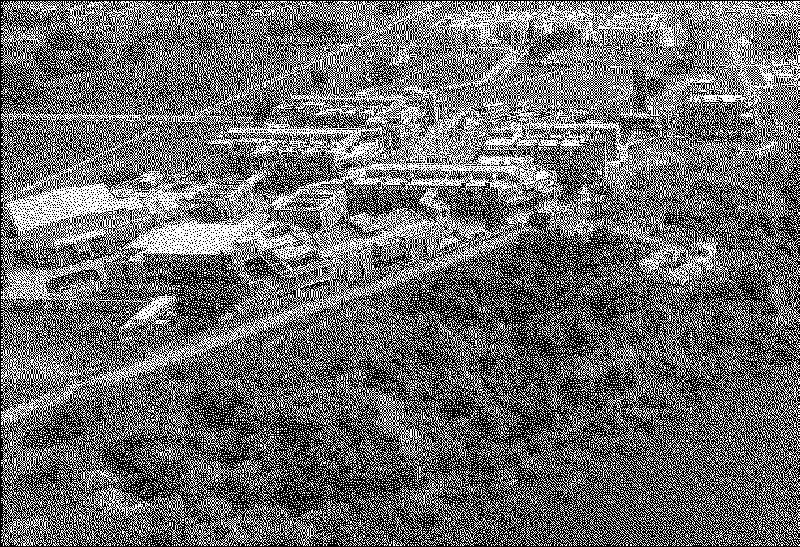
\includegraphics[width=0.75\linewidth]{41.png}
        \caption{Image after Error diffusion}
        \label{fig:Image after Error diffusion}
    \end{figure}
    \item Input Image $\longrightarrow$ 1{\_}user
    %%%%%%%%%%%
    \[
    \alpha=
    \begin{bmatrix} 
     0.3553 &	83.5323 &	81.5369 &	96.4339 &	-110 &	0.0003
    \end{bmatrix}
    \]
    \begin{figure}[H]
        \centering
        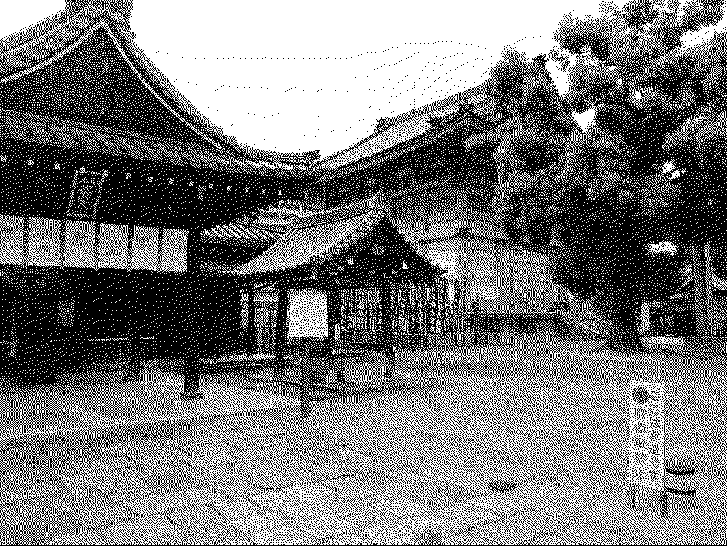
\includegraphics[width=0.75\linewidth]{42.png}
        \caption{Image after Error diffusion}
        \label{fig:Image after Error diffusion}
    \end{figure}
        \item Input Image $\longrightarrow$ 2{\_}user
        %%%%%%%%%%%%%%
        \[
    \alpha=
    \begin{bmatrix} 
      0.2924 &	94.7623 &	95.9311 &	100.4578 &	182	 & 0.0003
    \end{bmatrix}
    \]
    \begin{figure}[H]
        \centering
        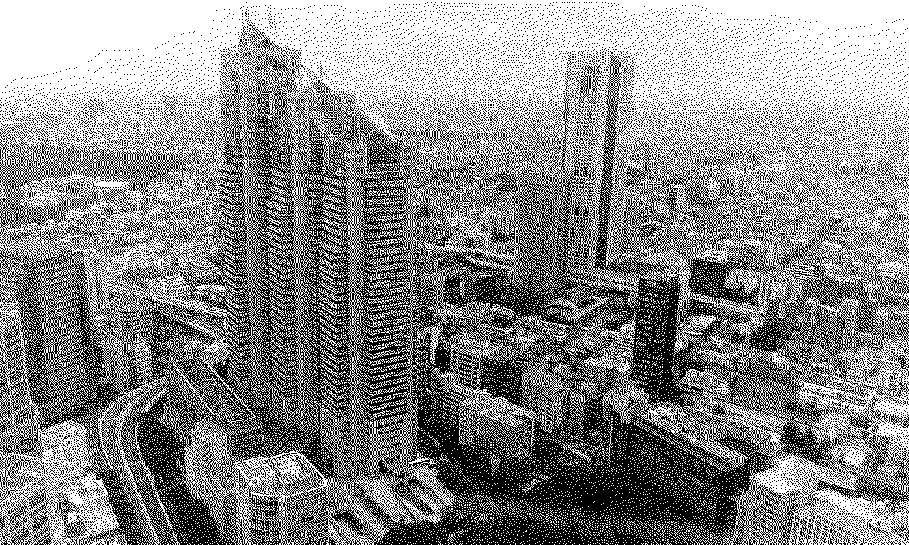
\includegraphics[width=0.75\linewidth]{43.png}
        \caption{Image after Error diffusion}
        \label{fig:Image after Error diffusion}
    \end{figure}
        \item Input Image $\longrightarrow$ 3{\_}user
        %%%%%%%%%%%%%%%%
        \[
    \alpha=
    \begin{bmatrix} 
      0.3875 &	85.9201 &	89.0826 &	93.4100 &	-22	& 0.0001
    \end{bmatrix}
    \]
    \begin{figure}[H]
        \centering
        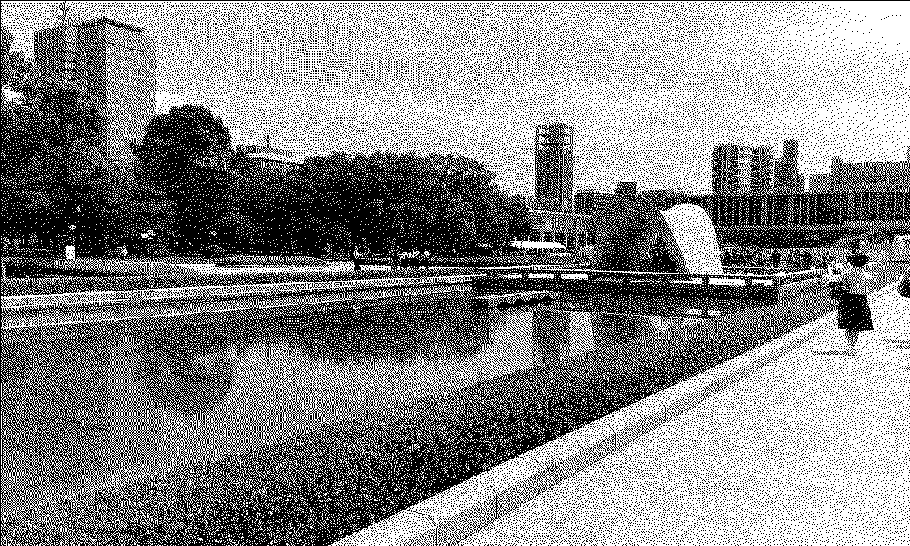
\includegraphics[width=0.75\linewidth]{44.png}
        \caption{Image after Error diffusion}
        \label{fig:Image after Error diffusion}
    \end{figure}
    \end{enumerate}
\end{document}
